% Poznámky dle komentářů supervizora, ad. konvence
	% po kódovém bloce novou větu
	% před blokem kódu konec věty může (ale nemusí) být,
		% avšak věta nesmí pokračovat za blokem
	% referování na funkce se složenými závorkami
		% -||-          makra s vykřičníkem
	% referování na nějaký kód -> nejsou-li speciální znaky,
		% poté monospace jen poprvé
	% před finalizací doformátovat nbsp přes `write_nbsp.py`

\documentclass[a4paper, 12pt, twoside]{article} % twoside
\usepackage[utf8]{inputenc} % utf-8 encoding
\usepackage[IL2]{fontenc} % ISO 8859-2

\usepackage[bf, sf]{titlesec} % formátování názvů
\newcommand{\sectionbreak}{\clearpage}

\usepackage{graphicx} % obrázky
\graphicspath{ {./static/} }
\usepackage{float} % správné pozice obrázků

\usepackage{geometry} % nastavení odsazení od krajů
\geometry{            %
	left=4cm,         %
	top=2.5cm,        %
	right=2.5cm,      %
	bottom=2.5cm      %
}                     %

\usepackage{nameref}
\usepackage{hyperref}   % odkazy
\usepackage{url}        %

\usepackage[nosingleletter]{impnattypo}

\usepackage{tocloft}        % manipulace TOC
\let\oldsection\section                                                     % tečkování TOC
\makeatletter                                                               %
\newcounter{@secnumdepth}                                                   %
\RenewDocumentCommand{\section}{s o m}{%                                    %
	\IfBooleanTF{#1}                                                          %
	{\setcounter{@secnumdepth}{\value{secnumdepth}}% Store secnumdepth      %
		\setcounter{secnumdepth}{0}% Print only up to \chapter numbers         %
		\oldsection{#3}% \section*                                             %
		\setcounter{secnumdepth}{\value{@secnumdepth}}}% Restore secnumdepth   %
	{\IfValueTF{#2}% \section                                               %
		{\oldsection[#2]{#3}}% \section[.]{..}                               %
		{\oldsection{#3}}}% \section{..}                                     %
}                                                                           %
\makeatother                                                                %

\setcounter{secnumdepth}{0} % 0 = žádné číslování sekcí

% ?
\usepackage{xparse}
\usepackage{setspace}

\usepackage{minted} % kód
\usepackage{xcolor} % barevný font
\usepackage{upquote}
\usepackage{xpatch} % vypnutí šikmého řezu v~minted blocích a inlines
\xpatchcmd{\mintinline}{\begingroup}{\begingroup\let\itshape\relax}{}{}
\xpatchcmd{\minted}{\VerbatimEnvironment}{\VerbatimEnvironment\let\itshape\relax}{}{}

\definecolor{mint_bg}{rgb}{0.975,0.975,0.975}
\definecolor{mint_bg_inline}{rgb}{1,1,1}
\setminted{bgcolor=mint_bg, fontsize=\footnotesize, baselinestretch=1, tabsize=4, breaklines, style=trac}

% zkratka pro inline kód
\newcommand{\rust}[1]{\mintinline[bgcolor=mint_bg_inline, breaklines, breakanywhere]{rust}{#1}} 
\newcommand{\bash}[1]{\mintinline[bgcolor=mint_bg_inline, breaklines, breakanywhere]{bash}{#1}} 

\usepackage{forest} % diagramy pro souborovou strukturu

%\renewcommand{\cftsecleader}{\cftdotfill{\cftdotsep}} % tečky v~TOC
%\doublehyphendemerits=1000000 %

\renewcommand{\contentsname}{Obsah} % správný titulek obsahu
\renewcommand{\figurename}{Obrázek} % správný titulek obrázků


\usepackage{indentfirst} % odsazení prvního řádku v~odstavcích

\renewcommand{\baselinestretch}{1.5}  % řádkování
\setlength{\parindent}{10mm}          % odsazení 1. řádku odstavců
\setlength{\parskip}{6pt}             % mezera mezi odstavci
\titlespacing\section{6pt}{0pt}{-\parskip}\relax       % mezera
\titlespacing\subsection{6pt}{0pt}{-\parskip}\relax    % pod tituly sekcí


\usepackage[czech]{babel}
\usepackage[superscript]{cite}
\addto\captionsczech{\renewcommand{\refname}{Seznam použité literatury}} % správný titulek zdrojů

%\usepackage[
%   backend=biber
%  ,style=iso-numeric
%  ,bibencoding=UTF8
%]{biblatex}
%\let\cite\parencite
%\bibliography{literatura}

\begin{document}
\thispagestyle{empty}
\begin{center}
	{\LARGE Střední škola spojů a~informatiky Tábor, Bydlinského 2474} \\[1.5cm]
	\textbf{\LARGE Tvorba aplikace v jazyce Rust} \\ [4cm]
	
\includegraphics[width=7cm]{logo_alt.png}
\end{center}

\vspace*{\fill}

\begin{flushleft}
	\large
	%\includegraphics[width=7cm]{a.png} 
	\textbf{Student: }Marek Smolík              \newline
	\textbf{Třída: }IT4                         \newline
	\textbf{Vedoucí práce: }Ing. Dana Almášiová \newline
	\textbf{Datum odevzdání práce: } 31.3.2022
\end{flushleft}
\vfill

\newpage
\thispagestyle{empty}
\vspace*{\fill}


\subsection*{Čestné prohlášení}
	\noindent \textit{Prohlašuji, že jsem předkládanou práci vypracoval sám za použití zdrojů a~literatury v~ní uvedených. Souhlasím s~tím, aby moje maturitní práce byla využívána pro potřeby Střední školy spojů a~informatiky Tábor, Bydlinského 2474 nebo jiných subjektů, které se podílely na~zadání práce.} \\[1.5cm]
	\noindent \makebox[3cm]{\dotfill} \hfill \makebox[3cm]{\dotfill} \newline
	\noindent datum \hfill podpis

\newpage

\tableofcontents

\newpage


\section*{Úvod}
	Rust je jedním z~nejrychleji se rozšiřujících programovacích jazyků. Jeho kompilér je otevřený software vyvíjený firmou Mozilla. Dle statistik webového portálu \href{https://stackoverflow.com/}{Stack Overflow} se jedná o  „Programátory nejoblíbenější jazyk“ dle všech hlasování v~rocích 2015-2021 konsekutivně \cite{stack}. Tomu je tak i~přes jeho relativní mladost. Má všestranně se rozšiřující ekosystém — lze v~něm programovat servery, vestavěné systémy, GUI, weby, ad. včetně systémového programování umožnénému díky jeho abstrakci s~nulovou cenou.

	Rust mě zaujal zejména díky velice dobrému hodnocení co se týče nižších programovacích jazyků, proto jsem si ho i~zvolil jako první jazyk této kategorie, který jsem se naučil.
	
	Tato práce si bere za cíl představit tento jazyk, jeho přednosti, výhody a~nevýhody. Její součástí je program v~jazyce vytvořený a~přílohy obsahují příručku — zevrubného a~rozsáhlého průvodce programováním v~jazyce Rust.

\section*{Seznámení s~Rustem}
	\subsection{Přehled a~využití}
		Rust je nízkoúrovňový kompilační jazyk vyvíjený společností Mozilla. Jeho \textit{de facto} cílem je být „modernější“ a~„bezpečnější“ C++. S~tímto jazykem má mnohé společné — má statickou typovou kontrolu, oba jsou objektově orientované, dovolují správu paměti na~nízké úrovni, atd. Dokonce některé Rustové programy jsou pouhými wrappery pro stávající C++ aplikace. Čím se však snaží tento letitý standard předčít je svojí paměťovou a~vláknovou bezpečností. Tu zaručuje jeho kompilér a~velice efektivně je tak zabráněno runtime chybám (takovým, vytvořeným během doby, při níž je samotný program spuštěn).

		Tato vlastnost je mezi programátory vysoce ceněna. Také dost stávajících projektů/standardů začalo integrovat Rust do svých produktů. Některé z~těchto společností jsou DropBox\cite{dropbox}, Cloudflare\cite{cloudflare}, npm\cite{npm}, Discord\cite{discord} a~četné množství dalších. Nejvýznamnější entitou zakomponovávající Rust je Amazon\cite{amazon}, který v~Rustu napsal celý jejich Firecracker VMM a~přispěl do ekosystému.

\section{Přednosti jazyka}
	\subsection{OOP}
		Podobně jako ve spoustě dalších jazyků nabízí Rust model pro objektově orientované programování. To je zprostředkováno pomocí struktur, nikoliv tříd. Výkonnostně jsou tyto metody velice podobné, liší se prakticky jen jejich programovacími rozhraními. Základním typem OOP je \texttt{enum}. Je to výčtový typ — tvoří ho libovolné množství pojmenovaných polí.
		\begin{minted}{rust}
enum Jazyk {
	Python,
	Rust
	WebAssembly,
}
		\end{minted}
		
		Následně lze instance těchto enumerací porovnávat pomocí vzorů řízení toku.
		\begin{minted}{rust}
fn main() {
	let muj_jazyk = Jazyk::Rust;
	
	if let Jazyk::Rust =  muj_jazyk {
		// ...
	}
	
	match muj_jazyk {
		Jazyk::Rust => { /* ... */ },
		Jazyk::Python => { /* ... */ },
		Jazyk::WebAssembly => { /* ... */ },
	}
	
}
		\end{minted}
		
		Avšak hlavní datastrukturou OOP v Rustu je struktura — \texttt{struct}. Ta, jak již bylo řečeno, je ekvivalentem tříd v jiných jazycích.
		\begin{minted}{rust}
struct Clovek {
	jmeno: String,
	prijmeni: String,
	vek: u8,
}
		\end{minted}
		
		Nadále lze použít \texttt{impl} pro tvorbu metod nad danou strukturou.
		\begin{minted}{rust}
impl Clovek {
	fn rekni_ahoj(&self) {
		println!(
			"Ahoj, jsem {} {} a je mi {} let.",
			self.jmeno,
			self.prijmeni,
			self.vek
		);
	}
}
		\end{minted}
		
		\subsubsection{Kompozice místo dědičnosti}
			Rust nemá třídy, ale struktury. Tyto struktury používají místo dědičnosti kompozici. Při tomto paradigmatu je využíváno shlukování sdílených vlastností více struktur. Tyto množiny se nazývají \texttt{trait}s. Identifukují sadu metod, které by měli \texttt{struct}y, které ji implementují, mít.
			\begin{minted}{rust}
trait Starnuti {
	fn zvysit_vek(&mut self);
}

struct Clovek {
	jmeno: String,
	prijmeni: String,
	vek: u8,
}

struct Zvire {
	jmeno: String,
	vek: String,
}

impl Starnuti for Clovek {
	fn zvysit_vek(&mut self) {
		self.vek += 1;
	}
} 
impl Starnuti for Zvire {
	// ...
}
			\end{minted}
		
		\subsubsection{Generika místo polymorfismu}
			Polymorfismus je způsob použití stejného rozhraní pro různé datové struktury. Toho lze v~Rustu dosáhnout pomocí využití generických funkcionalit.
			\begin{minted}{rust}
fn vypsat<T: Display>(arg: T) {
	println!("{}", T);
}
			\end{minted}
			
			Tento syntax značí, že funkce \texttt{vypsat()} využívá 1 generickou datovou strukturu, která musí implementovat \texttt{trait} \texttt{Display} (tato \texttt{trait} slouží pro vypsání hodnoty dané proměnné). Následně je poznamenáno, že argument \texttt{arg} je tohoto typu.
			
			Specifikování \texttt{trait}s, které daná datová struktura implementuje je nutné pro splnění statické kontroly typů.
			
			Kompilérem je na základě analýzy kódu zjištěno, přesně kterými typy je ve skutečnosti generická funkce využívána (na základě statické typové kontroly) a~následně funkci pro všechny tyto typy vygeneruje. Tomuto procesu se říká \textbf{monomorfizace}.

	\subsection{Modulový systém}
		Lokální soubory nejsou strukturovány manuálně. O tuto činnost se stará správce projektu \texttt{cargo}. Jde o systém podobný npm, což je správce projektů běžících pod systémem Node.js.
		
		Struktura cargem vygenerovaná po inicializaci projektu je následující
		\begin{center}
			\begin{forest}
				for tree={
				font=\ttfamily,
				grow'=0,
				child anchor=west,
				parent anchor=south,
				anchor=west,
				calign=first,
				edge path={
					\noexpand\path [draw, \forestoption{edge}]
					(!u.south west) +(7.5pt,0) |- node[fill,inner sep=1.25pt] {} (.child anchor)\forestoption{edge label};
				},
				before typesetting nodes={
					if n=1
					{insert before={[,phantom]}}
					{}
				},
				fit=band,
				before computing xy={l=15pt},
				}
			[muj\_projekt
				[.git
					[\vdots]
				]
				[src
					[main.rs]
				]
				[.gitignore]
				[Cargo.toml]
			]
			\end{forest}
		\end{center}
		
		Ve výchozím stavu, najde-li cargo při stavění projektu ve složce \texttt{src} soubor \texttt{main.rs}, považuje ho za root (kořen) projektu. Zároveň na~jeho základě vytvoří automaticky binární tzv. crate (ekvivalent package, tj. „balíčky“ u~jiných systémů). Pro rozšiřování projektu lze přidat do složky \texttt{src} soubor \rust{lib.rs}. Ten slouží jako knihovna — obsahuje kód pro využití ve více souborech, popřípadě odkazuje na~logické části adresáře. Je-li tento soubor cargem nalezen, je automaticky vytvořená druhá crate — library crate. Pravidlem je, že každý projekt musí být alespoň 1 crate — buďto library crate, nebo binary crate. Zároveň binárních může být libovolné množství, ale library může být maximálně jedna.

		Pokud je žádoucí více binárních crate (a tedy více vyprodukovaných binárních souborů), ve složce \texttt{src} potřeba vytvořit složku \texttt{bin}. Následně každý \texttt{.rs} soubor v~této složce umístěný bude cargem zvlášť zpracován jako binární crate a~každý z~nich při stavění vyprodukuje binární soubor. Toto však není příliš časté. Většinou je ve~složce \texttt{src} tvořeno více pomocných souborů, jejichž obsah je buďto implicitně, nebo explicitně volán přes kořenový soubor (\texttt{main.rs}). V~praxi postup takové tvorby může být následovný.
		\begin{center}
			\begin{forest}
				for tree={
				font=\ttfamily,
				grow'=0,
				child anchor=west,
				parent anchor=south,
				anchor=west,
				calign=first,
				edge path={
					\noexpand\path [draw, \forestoption{edge}]
					(!u.south west) +(7.5pt,0) |- node[fill,inner sep=1.25pt] {} (.child anchor)\forestoption{edge label};
				},
				before typesetting nodes={
					if n=1
					{insert before={[,phantom]}}
					{}
				},
				fit=band,
				before computing xy={l=15pt},
				}
			[src
				[main.rs]
				[lib.rs]
				[formatovani.rs]
			]
			\end{forest}
		\end{center}
		
		Obsah souborů podléhající této souborové struktuře by mohl být takovýto.
		\begin{minted}{rust}
// formatovani.rs

pub fn nahoru(s: String) -> String {
	return s.to_uppercase();
}

// lib.rs
pub mod formatovani;

// main.rs

mod formatovani;

fn main() {
	let a = "ahoj".to_string();
	
	println!("{}", formatovani::nahoru(s));
}
		\end{minted}

		První poznatkem zde je, že funkce v~odděleném souboru je označena klíčovým slovem \texttt{pub} to je potřebné z~toho důvodu, že by jinak nebyla dosažitelná z~ostatních modulů. V~Rustu jsou implicitně všechny datové struktury privátní a~pro využití v~jiné lokaci je nutno viditelnost explicitně označit.
		
		Následně je \texttt{formatovani.rs} nutno označit jako validní modul v~\texttt{lib.rs}. Poté ho již lze využít z~\texttt{main.rs}.
		
		\subsubsection*{std modul a~přidružené}
			Holý Rust má 5 základních crates, které jsou součástí každé instalace a~lze je využít i~v~prázdném projektu
			\begin{itemize}
				\item \textbf{alloc} - obsahuje většinu funkcionality pro alokaci a~správu paměti
				\item \textbf{core} - obsahuje základní funkcionality, jako primitivní typy
				\item \textbf{proc\_macro} - podpora pro definování vlastních (procedurálních) maker
				\item \textbf{std} - poskytuje abstrakci základní funkcionality pro cross-platform
				\item \textbf{test} - podpora testů a~výkonnostního testování
			\end{itemize}

			Některé z~nich, jako alloc a~core, jsou reexportovány v~std. Navíc část std je automaticky přidána do každého programu, jelikož by nebylo praktické importovat každý jeden komponent manuálně. Přesto některé prvky, které nejsou zbytné, jako \rust{std::collections::HashMap}, je nutno importovat.

		\subsubsection*{Externí crates}
			Stránka \href{https://crates.io/}{crates.io} je oficiálním internetovým repozitářem pro komunitní crates. K~24.1.2022 jich hostuje stránka na~75251 a~nejstahovanější crate je \href{https://crates.io/crates/rand}{rand}. V~pravé liště stránky vybrané crate lze vyčíst, že pro import lze použít syntax typu \texttt{crate = "verze"}. V~době citace je ekvivalentem pro tuto crate \texttt{rand = "0.8.4"}. Je-li ji chtěno v~projektu použít, vloží se tento text do souboru \texttt{Cargo.toml} do sekce \texttt{[dependencies]}.
			\begin{minted}[tabsize=4, breaklines]{toml}
[dependencies]
rand = "0.8.4"
			\end{minted}
		
			Alternativně lze importovat crates z~git repozitářů. Např.: pro regex by mohl vypadat takto:
			\begin{minted}{toml}
regex = { git = "https://github.com/rust-lang/regex", branch = "next" }
			\end{minted}

			Poté lze s~těmito moduly pracovat. Při prvním stavění projektu po přidání se tyto crates (a všechny ostatní crates, na~kterých projekt závisí) nejprve zkompilují (při dalších stavěních již toto není nutné).
			\begin{center}
				\begin{figure}[H]
					\centering
					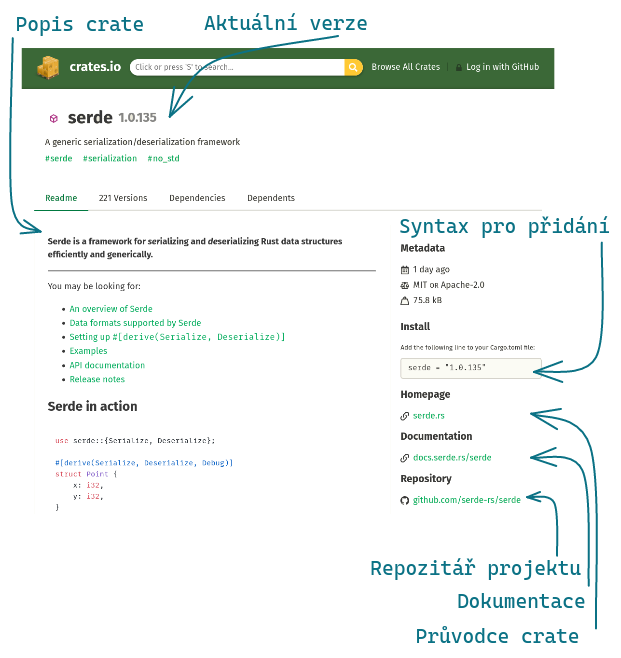
\includegraphics[width=0.95\linewidth]{cratesio}
					\caption{Ukázka a~popis crate serde na~\href{https://crates.io}{crates.io}}
					\label{fig:cratesio}
				\end{figure}
			\end{center}
			
			Avšak ještě je potřeba vědět, jak s~danou crate zacházet. Na~její stránce na~\href{https://crates.io}{crates.io} lze přečíst její popis, který většinou poskytuje minimalistickou ukázku kódu znázorňující zacházení s~ní. Avšak (pokud zde vůbec je) obsahuje minimální informace. Popřípadě, je-li crate komplexnější, může obsahovat jakéhosi průvodce, označeného v~pravé liště odrážkou \texttt{Homepage}.

		\subsubsection*{Dokumentace}
			Pro hlubší obeznámení s~jednotlivými crates je interakce s~přímou dokumentací nevyhnutelná. Není však nutné číst přímo zdrojový kód. Ekosystém poskytuje stránku \href{https://docs.rs}{docs.rs}, která autogeneruje nízkoúrovňovou dokumentaci přímo z~repozitářů. Lze zde najít i~\href{https://docs.rs/rustc-std-workspace-std/latest/std/index.html}{dokumentaci pro crate \rust{std}}. Například pro crate \rust{serde} vypadá takto
			\begin{center}
				\begin{figure}[H]
					\centering
					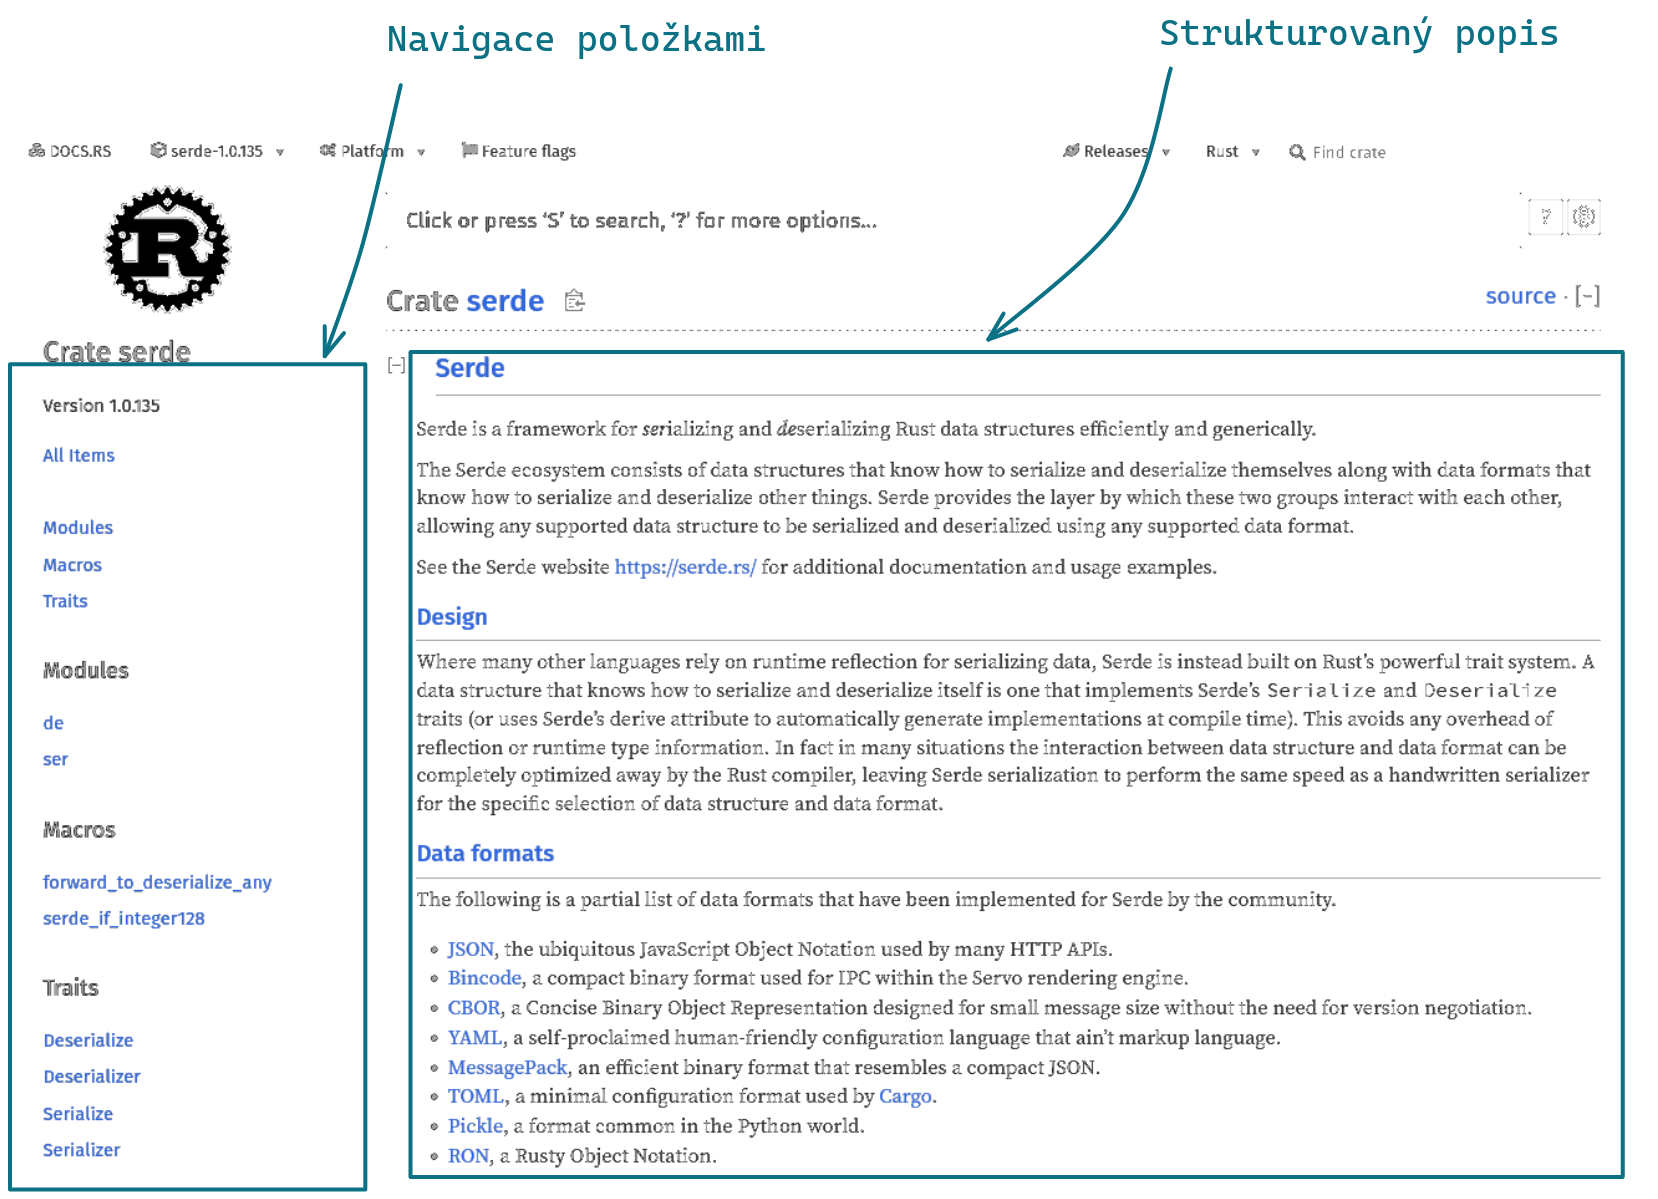
\includegraphics[width=\linewidth]{docsrs}
					\caption{Ukázka a~popis crate serde na~\href{https://docs.rs}{docs.rs}}
					\label{fig:docsrs}
				\end{figure}
			\end{center}

	\subsection{Model vlastnictví}
		\subsubsection*{Pravidla pro manipulaci paměti}
			Některé programovací jazyky jako Java, Haskell nebo Go mají garbage collector (odvoz odpadu). Ten uvolňuje pamět zabranou proměnnými právě, když vyjdou z~rámce, v~kterém jsou definovány a~proměnné jsou takto zinvalidněny. Jiné jazyky nic takového neposkytují a~paměť musí být spravována přímo programátorem. Takovým příkladem může být C. Rust se liší od těchto dvou skupin tím, že vnutí přesná pravidla a~postupy dané modelem vlastnictví, díky čemuž kompilér ví přesně, kdy proměnná má zaniknout, nebo skončí-li ji životnost (tzv. lifetime) a~na~základě toho použije adekvátní instrukce LLVM nebo jazyka symbolických adres (tento systém se označuje jako OBRM - ownership based resource management).

			\begin{center}
				\begin{figure}[H]
					\centering
					\includegraphics[width=.9\linewidth]{sprava_pameti}
					\caption{Různé strategie správy paměti \cite{sprava_pameti}}
					\label{fig:ret_mod}
				\end{figure}
			\end{center}
		
			Pro zachování bezpečnosti ohledně proměnných má Rust velice sofistikovaný a~specifický model vlastnictví. Je tomu tak, jelikož jeho filozofií je napsat o~něco více kódu, což se však záhy vyplatí redukcí runtime chyb.
	
			Tento model má několik pravidel, které musí být vždy dodržena.
			\begin{itemize}
				\item v~jakýkoliv daný moment smí mít proměnná buďto 1 mutable referenci, nebo libovolný počet immutable (neměnitelných) referencí
				\item reference musí vždy být validní (tj. nesmí odkazovat na~neexistující proměnné)
			\end{itemize}
			
			(Ve skutečnosti se tato pravidla avšak nevztahují na tzv. chytré ukazatele.) Dodržení těchto pravidel je při kompilaci zaručeno pomocí borrow checkeru (kontroléru půjčení).
			\begin{minted}{rust}
fn main() {
	let a = "a".to_string();
	
	let b = a;
	
	println!("{}", a);
}
			\end{minted}
	
			Tato ukázka kódu zámerně nezkompiluje. Borrow checker to nedovolí a~vrátí následující chybu
			\begin{minted}{bash}
error[E0382]: borrow of moved value: `a`
	--> src/main.rs:6:20
	|
2 |     let a = "a".to_string();
	|         - move occurs because `a` has type `String`, which does not implement the `Copy` trait
3 |     
4 |     let b = a;
	|             - value moved here
5 |     
6 |     println!("{}", a);
	|                    ^ value borrowed here after move
	|
	= note: this error originates in the macro `$crate::format_args_nl` (in Nightly builds, run with -Z macro-backtrace for more info)

				\end{minted}
					
				Ukazuje se, že ačkoliv kompilér Rustu (\texttt{rustc}) je velice striktní. Při chybě vrací přesná hlášení o~tom, co je špatně.

				Tento exaktní problém vyvstává z~toho, že vlastnictví hodnoty původně vlastněné proměnnou \texttt{a} bylo přesunuto proměnné \texttt{b}. V~tomto bodě je proměnná \texttt{a} zinvalidněna a~nelze ji nadále použít (pokud jí není přiřazena nová hodnota, kterou by byla schopna vlastnit). Tomuto lze předejít použitím referencí.
				\begin{minted}{rust}
fn main() {
	let a = "a".to_string();
	
	let b = &a;
	
	println!("{}", a);
}
				\end{minted}
		
				Tento případ se již zkompiluje, jelikož proměnná \texttt{b} pouze odkazuje na hodnotu proměnné \texttt{a}. Toto má jeden limit — hodnotu proměnné \texttt{b} takto nelze měnit. Pro tuto funkcionalitu by bylo nutno získat měnitelnou referenci, například takto
				\begin{minted}{rust}
fn main() {
	let mut a = "ahoj".to_string();
	
	let b = &mut a;
	println!("{}", b.to_uppercase()); // AHOJ

	// `a` je stále validní
	println!("{}", a); // ahoj
}
				\end{minted}
	
				Každá proměnná v~Rustu je ve výchozím stavu neměnitelná, proto ji je nutno definovat jako \texttt{mut} (mutable). Následně lze vytvořit měnitelnou referenci.
				
				S~referencemi však může někdy dojít k~problémům, je-li referováno na~hodnotu, která již neexistuje (byla uvolněná z~paměti)
				\begin{minted}{rust}
fn visici_ref() -> &String {
	let s = String::from("Jovan");

	return &s;
}

fn main() {
	let reference_na_nic = visici_ref();
}
				\end{minted}
				\cite{dangle}
					
				Tento příklad se nezkompiluje. Při spuštění funkce je vytvořena proměnná typu \rust{String}. Posléze se tato funkce snaží vrátit referenci na~hodnotu této proměnné, avšak při ukončení funkce je proměnná \texttt{s}~uvolněna z~paměti, a~tedy odkazovat na~ní nemá smysl (adresa v~paměti bude přepsána něčím jiným).
			
			\subsubsection*{Stack a~heap}
				Fundementálním konceptem je zde skutečnost, že při referování na proměnnou se nejedná o typ~\texttt{String}, kdežto se jedná o~\texttt{\&str} (string slice). Tento typ je jakýmsi pouhým náhledem do \texttt{String}u. Jedná se o to, že \texttt{String} je alokován na heap (haldu), kdežto \texttt{\&str} je na alokován na stack (zásobník).
				
				Stack je způsob ukládání dat do paměti, při kterém je daná hodnota nabita (push) na místo v~paměti s~konstantní velikostí a~posléze na~něj může být nabita další hodnota, nebo může být hodnota ze stacku vytlačena (pop). Avšak vždy lze operovat pouze s~hodnotou naposledy přidanou (tzv. LIFO model - Last In First Out).
				\begin{center}
					\begin{figure}[H]
						\centering
						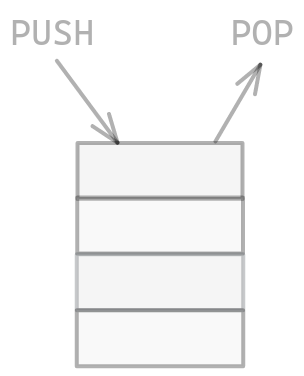
\includegraphics[width=4cm]{stack}
						\caption{Vizualizace správy paměti stack}
						\label{fig:my_label_2}
					\end{figure}
				\end{center}
	
				Druhým způsobem ukládání dat je heap. Ta je naopak od stacku používána pro hodnoty dynamicky měnící jako je \texttt{String} (a~datové struktury, jejichž celková velikost není známa při kompilaci). Je to jakýsi region paměti, ke kterému může být postupně přialokována (nebo odalokována) další paměť.

				Obecně se tyto dvě struktury liší rychlostí. Stack je znatelně rychlejší než heap, avšak nelze na~něj alokovat hodnoty neznámé velikosti.
	
				Kdykoliv je vytvořen řetězec, na~heap je přidán samotný obsah řetězce a~zároveň je na~stack přidán pointer (reference) odkazující na~adresu v~paměti, kde začíná řetězec) a~jeho délka (len)
					
				\begin{center}
					\begin{figure}[H]
						\centering
						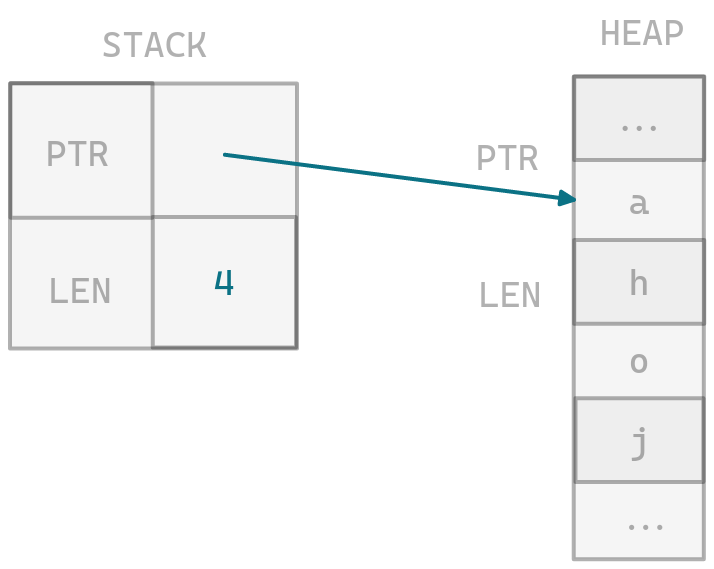
\includegraphics[width=6.5cm]{string_heap}
						\caption{Vizualizace vytvořeného řetězce znaků}
						\label{fig:my_label_3}
					\end{figure}
				\end{center}

				Část tohoto diagramu zobrazující stack je právě \rust{&str}. Toto je přesně typ, který je vracen inicializací jako \rust{let s = "ahoj"}. U~tohoto partikulárního příkladu je \rust{"ahoj"} pevně zakódovaný do binárního souboru vyprodukovaného po kompilaci a~při spuštění je načten do operační paměti.

			\subsubsection*{Dereferenční operátor}
				Občas může nastat situace, kdy je žádáno získat hodnotu proměnné přímo, ač může být schována za referencí. K~tomu lze využít dereferenční ho operátoru \rust{*}
				\begin{minted}{rust} 
let jovan = 7;
let navoj = &jovan;


// `navoj` s `jovan` nelze porovnat přímo,
// jelikož jsou jiných typů — i32 a &i32
if jovan == *navoj {
	/* ... */
}
				\end{minted}
		
			\subsubsection*{Lifetime}
				Lifetime (životnost) je vyjádřením doby, kterou daná proměnná žije. Buď demonstrací tento příklad s~visící referencí.
				\begin{minted}{rust}
fn main() {
	let t;

	{
		let u = 42;
		t = &u;
	}
	// pokud nejsou složené závorky {} nijak označené,
	// představují vlastní scope (rámec)

	// nic, co je vně těchto závorek, nemá přístup
	// k ničemu inicializovanému v tomto scope

	println!("{}", t);
}
				\end{minted}
				
				Tento příklad se nezkompiluje, jelikož by \rust{t} byla visící reference. Lifetimes proměnných \rust{t}, \rust{u} by vypadaly takto
				\begin{minted}{rust}
fn main() {
	let t;              // ---------+ 'a
						//          |
	{                   //          |
		let u = 42;     // -+ 'b    |
		t = &u;         //  |       |
	}                   // -+       |
						//          |
	println!("{}", t);  //          |
}                       // ---------+
			\end{minted}
			
				Lifetime \rust{t} je zde anotován jako \rust{'a} a~lifetime \rust{u} je anotován jako \rust{'b}. Diagram značí kde dané lifetimes začínají a~kde končí (tj. kde jsou proměnné zinvalidněny). Pomocí tohoto lze dovysvětlit visící referenci podrobněji — díky \rust{t = &u;} odkazuje \rust{t} na~\rust{u}, avšak \rust{u} nežije dostatečně dlouho na~to, aby mohla být využita její reference v~\rust{println!("{}", t);}.
				
				Konsekvencí lifetimes proměnných je nutnost jejich specifikace v~některých případech. Buď uvažován příklad
				\begin{minted}{rust}
fn nejvetsi(cislo1: &i32, cislo2: &i32) -> &i32 {
	if (cislo1 > cislo2) {
		cislo1
	} else {
		cislo2
	}
}

fn main() {
	let t = 7;
	let u = 42;
	
	println!("{}", nejvetsi(&t, &u));
}
				\end{minted}

				Toto se nezkompiluje, důvod je následující: výstupem funkce \rust{nejvetsi()} je odkaz na~jednu z~proměnných, které jsou referencovány v~jejích parametrech. Avšak z~pohledu borrow checkeru, který kontroluje lifetimes, není jasné, jaké mají tyto vstupní parametry lifetimes. Co kdyby vracel odkaz na proměnnou, která však nebude mít v~kontextu, ve kterém bude funkce použita, dostatečnou životnost? 
				
				Toto lze obejít anotací lifetimes v~hlavičce funkce \rust{nejvetsi}.
				\begin{minted}{rust}
fn nejvetsi<'a>(cislo1: &'a i32, cislo2: &'a i32) -> &'a i32
				\end{minted}
			
				Tato syntaxe říká, že lifetime výstupní hodnoty bude stejný jako nejmenší lifetime proměnných, na~něž je odkazováno pomocí \rust{cislo1} a  \rust{cislo2}.
				
				Toto není samozřejmě jediný postup anotace. Ten se upraví dle způsobu, jakým má být funkce použita. Například pokud by bylo žádoucí svázat lifetime výstupu funkce s~lifetime jedného z~parametrů, šlo by to následovně.
				\begin{minted}{rust}
fn jovan<'a, 'b>(i: &'a mut str, j: &'b i32) -> &'b i32
				\end{minted}
			
				Lifetime anotace dovoluje také tvorbu \texttt{struct}ů, které nevlastní hodnoty svých polí
				\begin{minted}{rust}
struct Jovan {
	navoj: &str,
}

fn main() {
	let s = "abc";
	
	let i = Jovan {
		navoj: s
	};
	
	println!("{}", i.navoj);
}
				\end{minted}
			
				Toto by se nezkompilovalo, avšak po následné modifikaci ano.
				\begin{minted}{rust}
struct Jovan<'a> {
	navoj: &'a str,
}
				\end{minted}

\section{Cross-platform export aplikací}
	Jedna ze zásad Rustu je být lehce použitelný na~kterékoliv běžné platformě, včetně vestavěných systémů.
	
	Dostupnost možných kompilovacích cílů lze zjistit následovně
	\begin{minted}{shell}
rustc --print target-list
	\end{minted}
		
	V~současné době tento list vrátí asi 175 možných cílů. Ty zahrnují architektury jako x86\_64, aarch64, arm, i686, wasm32, a~četné množství dalších pro systémy jako Windows, GNU/Linux, BSD, Android, MacOS a~další. Pro export do kterékoliv z~těchto cílů je však nejprve nutno stáhnout sadu pro danou architekturu. Například pro x86\_64-pc-windows-gnu by příkaz vypadal následovně
	\begin{minted}{shell}
rustup target add x86_64-pc-windows-gnu
	\end{minted}
	
	Dále pro přehled všech instalovaných cílů lze použít
	\begin{minted}{shell}
rustup target list
	\end{minted}

	\subsection{Windows}
	Windows obecně nevyužívá žádné kontejnerizace aplikací, díky čemuž je export poměrně jednoduchý.
	
	\subsubsection*{Přídání ikony binárního souboru}
		Pro přidání ikony lze využít crate \texttt{winres}. Nejprve je nutno ji přidat do \texttt{Cargo.toml}
		\begin{minted}{bash}
[target.'cfg(windows)'.build-dependencies]
winres = "0.1"
		\end{minted}
		
		Význam pole \texttt{[target.'cfg(windows)'.build-dependencies]} spočívá v~přidávání crates, které mají být importovány pokud je kompilováno s~cílovou platformou Windows.
		
		Dále je potřeba přidat do stejného adresáře speciální soubour \texttt{build.rs}. Tento soubor slouží pro pokročilejší manipulaci při kompilaci. Jeho obsah bude následující
		\begin{minted}{rust}
fn main() -> std::io::Result<()> {
	#[cfg(windows)] {
		winres::WindowsResource::new()
			.set_icon("resources/icon.ico")
			.compile()?;
	}
	Ok(())
}
		\end{minted}

		Zde je využito podmíněné kompilace — pro rozhodnutí, zda-li má daná sekce být zkompilována, je využito nějakého logického výrazu, v~tomto případě \mintinline{rust}{#[cfg(windows)]}. Nadále v~tomto úryvku \rust{"resources/icon.ico"} je cesta k~ikoně relativní vůči adresáři se souborem \texttt{Cargo.toml}.\cite{comp_win_ico}.
		
		Následně, pokud aplikace využívá GUI, lze do souboru \texttt{main.rs} přidat následující
		\begin{minted}{rust}
#![windows_subsystem = "windows"]
		\end{minted}
		
		Toto zaručí, že se společně s~GUI neotevře okno s~příkazovým řádkem. Následuje
		\begin{minted}{bash}
cargo build --release --target=x86_64-pc-windows-msvc
		\end{minted}
		
		A tím je program postaven, výsledkem je binární \texttt{.exe} soubor.\cite{winexport}


	\subsection{GNU/Linux}
		Linux je poněkud složitější co se týče exportu, to je dáno tím, že preferabilně jsou aplikace distribuovány kontejnerizované. V~následujícím příkladu je popsána tvorba aplikace kontejnerizované dle standardu AppImage. Tento formát je široce rozšířený, má oficiální podporu na~distribucích jako Arch Linux, Ubuntu, Debian, ad.\cite{appimage}

		Nejprve se aplikace zkompiluje, např. pomocí
		\begin{minted}{bash}
cargo build --release --target x86_64-unknown-linux-gnu
		\end{minted}

		Poté je nutno vytvořit dočasnou složku
		\begin{minted}{bash}
mkdir temp.AppDir
		\end{minted}
		
		Následně se do této složky nakopíruje binární soubor a~jeho ikona
		\begin{minted}{bash}
cp target/x86_64-unknown-linux-gnu/release/muj_program temp.AppDir/AppRun
cp resources/icon.png temp.AppDir/
		\end{minted}
		
		V~neposlední řadě je nutno v~této složce vytvořit soubor s~manifestem obsahující metadata
		\begin{minted}{bash}
echo "
[Desktop Entry]
Name=Muj_program
Exec=muj_program
Icon=icon.png
Type=Application
Categories=Game;
" > temp.AppDir/Muj_program.desktop
		\end{minted}

		Takto je již aplikace připravená a~lze použít např. nástroje appimagetool\cite{appimagetool}
		\begin{minted}{bash}
appimagetool temp.Appdir
		\end{minted}

		Tímto dojde k~vytvoření souboru \texttt{Muj\_program.AppImage}, který lze distribuovat.

	\subsection{WebAssembly}
		WebAssembly (WASM) je technologie umožňující spuštění výpočetně náročných aplikací ve webovém rozhraní. Toho je dosáhnuto tak, že kód nějakého jazyka (preferabilně nízkoúrovňového) je přeložen do \texttt{.wasm} bajtkódu. Pokud tedy aplikace potřebuje vysoký výkon pro nějaký úkon, může ho JavaScriptové API přenechat tomuto WASM bajtkódu.\cite{wasm}
		
		\begin{center}
			\begin{figure}[H]
				\centering
				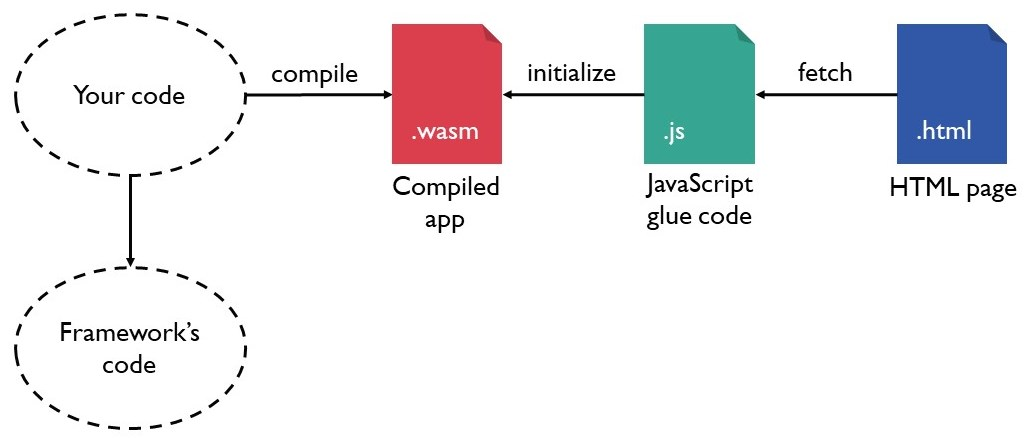
\includegraphics[width=13cm]{wasm}
				\caption{Proces využití WebAssembly pro webové aplikace \cite{wasm_fig}}
				\label{fig:wasm}
			\end{figure}
		\end{center}
		
		Postup pro získání bajtkódu i~lepícího kódu (který bude komunikovat mezi JS a~bajtkódem) lze postupovat následovně.
		
		Nejprve je potřeba přidat dependencies do \texttt{Cargo.toml}
		\begin{minted}{toml}
[target.'cfg(target_arch = "wasm32")'.dependencies]
tracing = "0.1.29"
tracing-subscriber = "0.2.25"
tracing-wasm = "0.2.0"
		\end{minted}
		
		Užitý syntax má význam v~přidávání crates specifických pro cílovou architekturu \texttt{wasm32}. Crate \texttt{tracing} není povinná, ale nastane-li chyba ze strany wasm bajtkódu, je schopna tuto chybu vypsat do vývojářské konzole webového rozhraní (DevTools). Posléze je nutno poskytnou speciální funkci, která bude vstupním bodem pro wasm
		\begin{minted}{rust}
#[cfg(target_arch = "wasm32")]
#[wasm_bindgen]
pub fn main_web(canvas_id: &str) {
	tracing_wasm::set_as_global_default();

	// *kód pro spuštění na webu*
}
		\end{minted}
		
		Nyní jen zbývá přidat následující do \texttt{Cargo.toml}
\begin{minted}{toml}
[lib]
crate-type = [ "cdylib", "rlib" ]
		\end{minted}
		
		A nyní už je hotovo po stránce editování původního kódu a~lze přejít ke kompilování.
		\begin{minted}{bash}
cargo build --release --lib \
			-p muj_program \
			--target wasm32-unknown-unknown \
		\end{minted}
		
		Následně je potřeba vygenerovat glue code. K~tomu lze použít programu \texttt{wasm-bindgen}. Ten se dá nainstalovat přes
		\begin{minted}{bash}
cargo install -f wasm-bindgen-cli
cargo update -p wasm-bindgen
		\end{minted}
		
		Poté ho lze použít na~vygenerovaný WASM soubor
		\begin{minted}{bash}
wasm-bindgen target/wasm32-unknown-unknown/release/muj_program.wasm \
			--no-modules \
			--no-typescript \
		\end{minted}
		
		Toto v~adresáři WASM souboru vygeneruje soubor \texttt{muj\_program\_bg.js}. Nyní se vezme tento soubor společně s~\texttt{muj\_program.wasm} a~oba jsou přesunuty do nové složky. V~této samé složce je nutno vytvořit HTML soubor, např. \texttt{index.html}, s~následujícím obsahem
		\begin{minted}{html}
<!DOCTYPE html>
<html>
<head>
	<title>Hra života</title>
</head>
<body>
	<canvas id="app"></canvas>

	<script src="muj_program_bg.js"></script>
	<script>
		wasm_bindgen("./muj_program.wasm")
			.then(on_wasm_loaded)
			.catch(console.error);

		function on_wasm_loaded() {
			wasm_bindgen.main_web("app");
		}
	</script>
</body>
</html>
		\end{minted}
		
		Díky minimálnímu kódu je načten bajtkód a~spuštěna dříve definované funkce \rust{main_web()} odkazující na~\texttt{canvas}, do kterého je GUI vykreslováno.
		
		Nyní však ještě není hotovo. Po otevření \texttt{index.html} ve webovém prohlížeči nebude aplikace fungovat. Při otevření konzole lze identifikovat vadu - CORS (Cross-origin resource sharing). Toto dává smysl — při pohledu na~soubor \texttt{index.html} lze zjistit, že funkce \rust{wasm_bindgen()} potřebuje načíst soubor \texttt{muj\_program\_bg.wasm} toto však nelze, nejsou-li soubory získány přes webový server. Jeden způsob by byl instalací webového serveru, například \texttt{basic-http-server}
		\begin{minted}{bash}
cargo install basic-http-server
		\end{minted}
		
		Ten lze využít (v adresáři s~webovými soubory) příkazem
		\begin{minted}{bash}
basic-http-server --addr 127.0.0.1:3000 .
		\end{minted}
		
		Nyní je celý proces hotov a~webovou aplikaci lze spustit z webového rozhraní na~zpětné adrese \texttt{127.0.0.1:3000}.\cite{wasm_vid, wasm_gh}

\section{Hra života s~GUI}
	\subsection{Vymezení cílů}
		Cílem této aplikace je naprogramovat cross-platform řešení pro uživatelem přizpůsobitelnou simulaci Hry života Johna Conwaye. Jedná se o „hru jednoho hráče“, která je vizualizována jako dvojrozměrné pole buněk. Každá tato buňka je v~jakémkoliv čase právě v~jednom ze dvou stavů — mrtvá nebo živá. Čas v~simulaci je kvantifikován na~tzv. generace. To, zda mrtvá buňka v~další generaci oživne, nebo to, zda-li živá buňka zemře, podléhá nastaveným pravidlům hry, které se vážou na~počet živých sousedních buněk. Tradiční konfigurace se označuje jako S23/B3. To znamená, že aby živá buňka přežila, musí mít 2 nebo 3 živé sousedy a~aby mrtvá buňka oživla, musí mít právě 3 živé sousedy (nastane-li cokoliv jiného, poté buňka umře, respektive zůstává mrtvá).\cite{conway}.
		\begin{center}
			\begin{figure}[H]
				\centering
				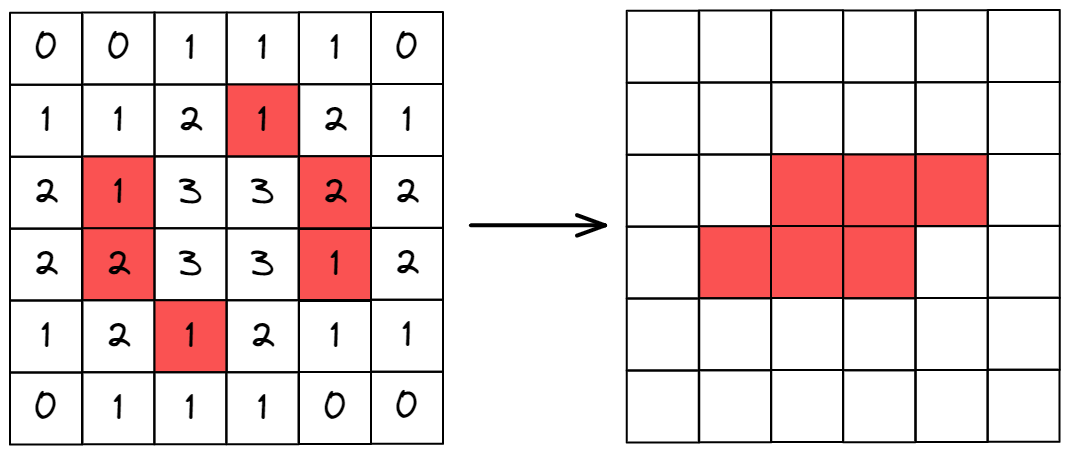
\includegraphics[width=.82\linewidth]{conway}
				\caption{Příklad vytvoření nové generace v~Conwayově Hře života, S23/B3}
				\label{fig:conway}
			\end{figure}
		\end{center}
	
		Aplikace by měla běžet na~všech signifikantních platformách a~měla by mít minimální systémové požadavky.
	
	\subsection{Výběr frameworku}
		Bohužel co se GUI frameworků týče, ekosystém Rustu ještě není dostatečně vybaven. Obecně není příliš velký výběr, všechny jsou immediate mode. Respektive existují ve vývoji i~retained mode, avšak ty jsou ve velice útlém a~experimentálním stádiu.

		Rozdíl mezi těmito dvěma je ten, že retained mode GUI si uchovává informace o rozvržení okna aplikace, a~tedy je toto okno přerenderováno pouze tehdy, je-li v~jeho vzhledu detekována nějaká změna. Kdežto immediate mode GUI si neuchovává nic a~každý jeden snímek je znovu renderován. Na~základě těchto poznatků lze vyvodit, že pokud se vzhled okna má často měnit (jako třeba nějaká hra), poté je vhodnější immediate mode, kdežto u~desktopových aplikací, jejichž vzhled se příliš nemění (jako třeba nějaké formuláře), je vhodnější retained mode. Tato aplikace má být něco mezi těmito dvěma paradigmaty, a~tedy limit daný omezeným výběrem není tak veliký problém.
		\begin{center}
			\begin{figure}[H]
				\centering
				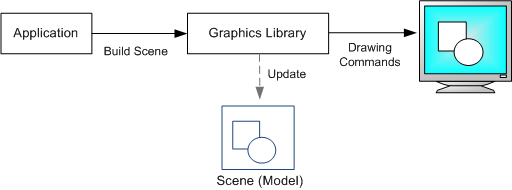
\includegraphics[width=.82\linewidth]{imm_mod}
				\caption{Diagram procesu renderování immediate mode\cite{imm_mod}}
				\label{fig:imm_mod}
			\end{figure}
		\end{center}
		\begin{center}
			\begin{figure}[H]
				\centering
				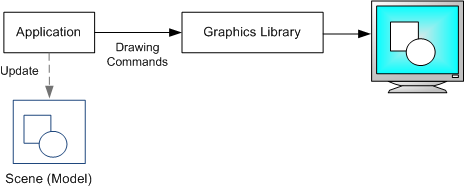
\includegraphics[width=.82\linewidth]{ret_mod}
				\caption{Diagram procesu renderování retained mode\cite{ret_mod}}
				\label{fig:ret_mod}
			\end{figure}
		\end{center}
		
		Frameworkem, který jsem nakonec zvolil je egui, a~to zejména kvůli tomu, že disponuje všemi funkcionality, které potřebuji - vykreslováním všech widgetů, které chci a~má excelentní podporu pro WebAssembly.\cite{egui}
	
	\subsection{Struktura / rozvržení}
		Po vytvoření projektu pomocí \texttt{cargo new gol} je vytvořeno několik dalších složek a~souborů tak, že struktura souborů bude vypadat následovně:
		\begin{center}
		\begin{forest}
			for tree={
			font=\ttfamily,
			grow'=0,
			child anchor=west,
			parent anchor=south,
			anchor=west,
			calign=first,
			edge path={
				\noexpand\path [draw, \forestoption{edge}]
				(!u.south west) +(7.5pt,0) |- node[fill,inner sep=1.25pt] {} (.child anchor)\forestoption{edge label};
			},
			before typesetting nodes={
				if n=1
				{insert before={[,phantom]}}
				{}
			},
			fit=band,
			before computing xy={l=15pt},
			}
		[gol
			[.git
			[\vdots]
			]
			[code
			[resources
				[logo.png]
			]
			[src
				[main.rs]
				[lib.rs]
			]
			[target
				[\vdots]
			]
			[Cargo.toml]
			]
			[dest
			[]
			]
			[.gitignore]
			[build.py]
		]
		\end{forest}
		\end{center}

		\begin{itemize}
			\item \texttt{code} slouží pro zdrojový kód a~související zdroje
			\begin{itemize}
				\item \texttt{resources} slouží pro obrázky, které program využívá
			\end{itemize}
			\item \texttt{dest} slouží pro exportované aplikace
			\item \texttt{build.py} je skript pro export aplikací
		\end{itemize}
		
	\subsection{Logická struktura}
		Jak je u~větších projektů zvykem, samotný soubor \texttt{main.rs} je jakousi pouhou „vstupní bránou“, která pouze inicializuje program. 
		
		\begin{minted}{rust}
use eframe::{run_native, NativeOptions};

// Game struct v lib.rs
use gol::Game;

fn main() {
    // import GUI iniciátorů
    use eframe::{run_native, NativeOptions};
    // import z knihovny
    use gol::Game;
    
    // `tracing` slouží pro hlášení informací
    tracing_subscriber::fmt::init();

    let game = Game::new();
    
    let win_option = NativeOptions::default();
    // spuštění GUI
    run_native(Box::new(game), win_option);
}
		\end{minted}
		
		Čiže se jen odkáže na~položky v~jiných modulech, v~tomto případě v~\texttt{lib.rs}. V~něm bude struktura následující
		\begin{minted}{rust}
// import lokálních souborů
mod config;
use config::Config;

// import komunitních beden
use eframe::{ /* ... */ };

// objekt buňky
#[derive(Default, Clone)]
struct Cell {
	pub is_alive: bool,
}

// herní objekt
pub struct Game {
	/* ... */
}

impl Game {
	// --------------------------------------
	//      Tvorba
	// --------------------------------------

	// pomocná funkce pro generování reprezentace pole s buňkami
	fn generate_board(size: usize) -> Vec<Vec<Cell>> { /* ... */ }

	// vytvoření instance hry
	pub fn new(size: usize) -> Game { /* ... */ }

	// --------------------------------------
	//      Manipulace
	// --------------------------------------

	// umožní změnit velikost hrací desky do spec. velikosti
	pub fn resize_to(&mut self, size: usize) { /* ... */ }

	// nastaví náhodný stav buněk
	pub fn randomize_cells(&mut self, factor: u8) { /* ... */ }

	// změní stav specifikované buňky
	pub fn change_cell_state(&mut self, cell: (usize, usize)) { /* ... */ }

	// vrátí pozici (ne)kliknuté buňky
	fn get_clicked_cell(&self, pos: Pos2, rect: Rect) -> Option<(usize, usize)> { /* ... */ }

	// --------------------------------------
	//      Herní logika
	// --------------------------------------

	// získá počet živých sousedů buňky
	fn get_neighbor_count(&self, pos: (i32, i32)) -> u8 { /* ... */ }

	// vytvoří novou desku na základě pravidel
	pub fn iterate(&mut self) { /* ... */ }

	// --------------------------------------
	//      Kontroléry, komunikace s GUI
	// --------------------------------------

	// rozhodování o možnosti další iterace v závislosti na konf.
	pub fn handle_iterate(&mut self, ui: &mut Ui) { /* ... */ }

	// přidělí místo pro pole s buňkami
	fn allocate_space_for_cells(&self, ui: &mut Ui) -> (Id, Rect) { /* ... */ }

	// vykresluje pole s buňkami
	fn show_cells(&mut self, ui: &mut Ui, rect: Rect) { /* ... */ }
}

// egui vyžadouje implementaci `App` pro daný herní objekt
impl App for Game {
	// vykreslování
	fn update(&mut self,
				ctx: &eframe::egui::CtxRef,
				_frame: &mut eframe::epi::Frame<'_>){
		egui::CentralPanel::default().show(ctx, |ui| { /* ... */ });
	}

	// název okna
	fn name(&self) -> &str { "Hra života" }
}
		\end{minted}

		Pro herní \texttt{struct} je tedy implementována požadovaná \rust{trait} \rust{App}, které vyžaduje dvě metody. Zbylé implementované metody souvisejí s~logikou hry a~její funkčností. Zde však není vše, je také zapotřebí pár úprav pro WebAssembly. Konkrétně je nejprve nutno nahradit 2 funkcionality - sledování času a~generování náhodných čísel. Pro tyto dva úkony jsou ve výchozím stavu užívány crates \rust{std::time} a~externí crate \rust{rand} v~tomto pořadí. Ty je nutno nahradit WebAssembly podporujícími alternativami.
		\begin{minted}{rust}
#[cfg(not(target_arch = "wasm32"))]
use std::time::{SystemTime, UNIX_EPOCH};
#[cfg(target_arch = "wasm32")]
use wasm_timer::{SystemTime, UNIX_EPOCH};
		\end{minted}
		
		Ještě je nutno označit v~\texttt{Cargo.toml} \texttt{lib} pro podporu WASM
		\begin{minted}{rust}
[lib]
crate-type = [ "cdylib", "rlib"]
		\end{minted}
		
		Tato část by byla hotova a~již stačí vytvořit vstupní bod pro WebAssembly (tj. funkci, na~kterou se JavaScript gluecode napojí)
		\begin{minted}{rust}
#[wasm_bindgen]
pub fn main_web(canvas_id: &str) {
    extern crate console_error_panic_hook;
    use std::panic;
    tracing_wasm::set_as_global_default();
    panic::set_hook(Box::new(console_error_panic_hook::hook));

    let game = Game::new();

    eframe::start_web(canvas_id, Box::new(game));
}
		\end{minted}
		
		Již zbývá poslední krok — nastavit ikonu pro Windows pomocí \rust{winres} v~souboru \texttt{build.rs}
		\begin{minted}{rust}
fn main() -> std::io::Result<()> {
	#[cfg(windows)] {
	winres::WindowsResource::new()
		.set_icon("resources/logo.ico")
		.compile()?;
	}

	Ok(())
}
		\end{minted}
		
		A nastavit, aby se na~Windows neotevíralo okno příkazového řádku, tedy přidat do hlavičky.
		\begin{minted}{rust}
#![windows_subsystem = "windows"]
		\end{minted}

\section{Závěr}
	Rust je velice dobrým programovacím jazykem a~osobně jsem si ho oblíbil. Ačkoliv má poměrně strmou učící křivku, má velice přívětivou komunitu vývojářu, kteří jsou ochotni pomoci. Dalším nedostatkem je relativní nevyspělost ekosystému a~nejspíše bude trvat ještě přinejmenším několik let, než bude mít Rust takové množství kvalitiních frameworků a~nástrojů, které mají některé jiné programovací jazyky. Toto je však dle mého názoru vše, co lze vytknout.
	
	V průběhu této práce jsem si upevnil svoji znalost jazyka Rust a~naučil jsem se pracovat s~novým grafickým frameworkem. Největší obtíže mi působilo vymyšlení podléhajících algoritmů.
	
	Jakožto přílohu přikládám vypracovanou příručku — zevrubného průvodce pro započetí programování v~Rustu.

\bibliographystyle{unsrt}
\bibliography{literatura}

\end{document}
	